\documentclass{article}
\usepackage{tikz}
\usetikzlibrary{3d}

\begin{document}

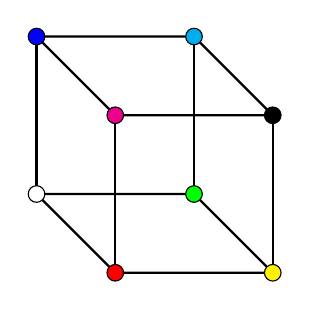
\begin{tikzpicture}[x={(0.5cm,-0.5cm)}, y={(1cm,0cm)}, z={(0cm,1cm)}]

% Define the coordinates of the cube
\coordinate (A) at (0,0,0);
\coordinate (B) at (2,0,0);
\coordinate (C) at (2,2,0);
\coordinate (D) at (0,2,0);
\coordinate (E) at (0,0,2);
\coordinate (F) at (2,0,2);
\coordinate (G) at (2,2,2);
\coordinate (H) at (0,2,2);

% Draw the back face
\draw[thick] (D) -- (C) -- (B) -- (A) -- cycle;

% Draw the front face
\draw[thick] (E) -- (F) -- (G) -- (H) -- cycle;

% Connect the front and back faces
\draw[thick] (A) -- (E);
\draw[thick] (B) -- (F);
\draw[thick] (C) -- (G);
\draw[thick] (D) -- (H);

% Add colored circles with black outlines at the vertices
\draw[black, fill=white] (A) circle (3pt);
\draw[black, fill=red] (B) circle (3pt);
\draw[black, fill=yellow] (C) circle (3pt);
\draw[black, fill=green] (D) circle (3pt);
\draw[black, fill=blue] (E) circle (3pt);
\draw[black, fill=magenta] (F) circle (3pt);
\draw[black, fill=black] (G) circle (3pt);
\draw[black, fill=cyan] (H) circle (3pt);

\end{tikzpicture}

\end{document}
